%==================================================================================
\begin{frame}
\frametitle{1966 - ASCII art appears}
\begin{columns}
    \begin{column}{0.45\textwidth}
        \centering
        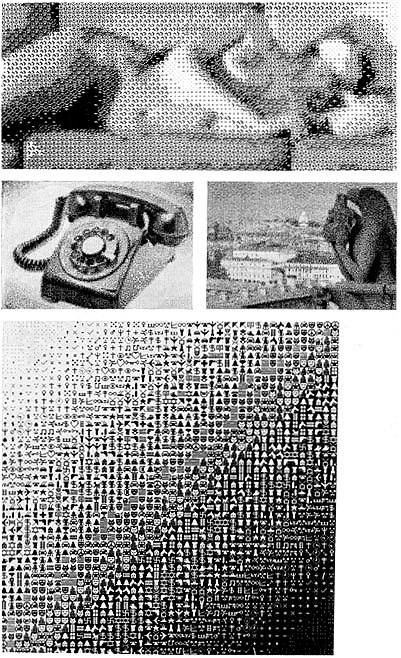
\includegraphics[width=\linewidth]{assets/bell.jpg}
    \end{column}

    \begin{column}{0.45\textwidth}
        Kenneth Knowlton, who worked at Bell Labs, created some of the earliest ASCII art known. He shared the images through a publication called "Studies in Perception I".
    \end{column}
\end{columns}
\end{frame}
%==================================================================================
%https://ralphbaer.com/TypedNotes_page.htm
\begin{frame}
\frametitle{1966 - Conceptual, TV Gaming Display}
\begin{columns}
    \begin{column}{0.45\textwidth}
        \centering
        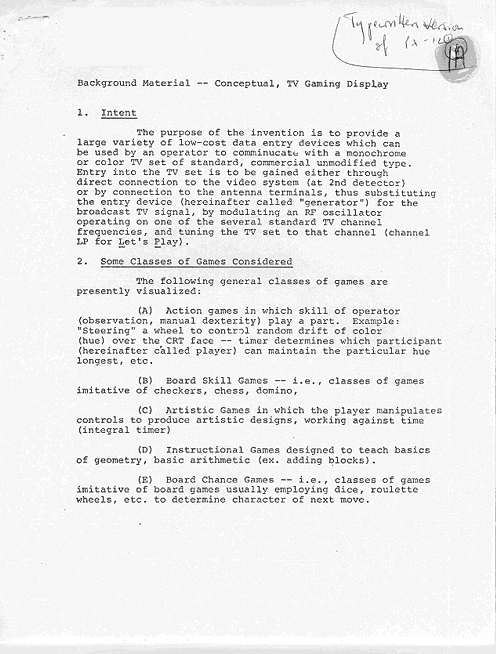
\includegraphics[width=\linewidth]{assets/baer.png}
    \end{column}

    \begin{column}{0.45\textwidth}
        Ralph Baer, a game developer and engineer, published an article showcasing a concept of how a monochrome or color monitor could be used for developing games, as well as some possible game types as examples.baer
    \end{column}
\end{columns}
\end{frame}
%==================================================================================
\begin{frame}
\frametitle{1966 - First HMD}
\begin{columns}
    \begin{column}{0.45\textwidth}
        \centering
        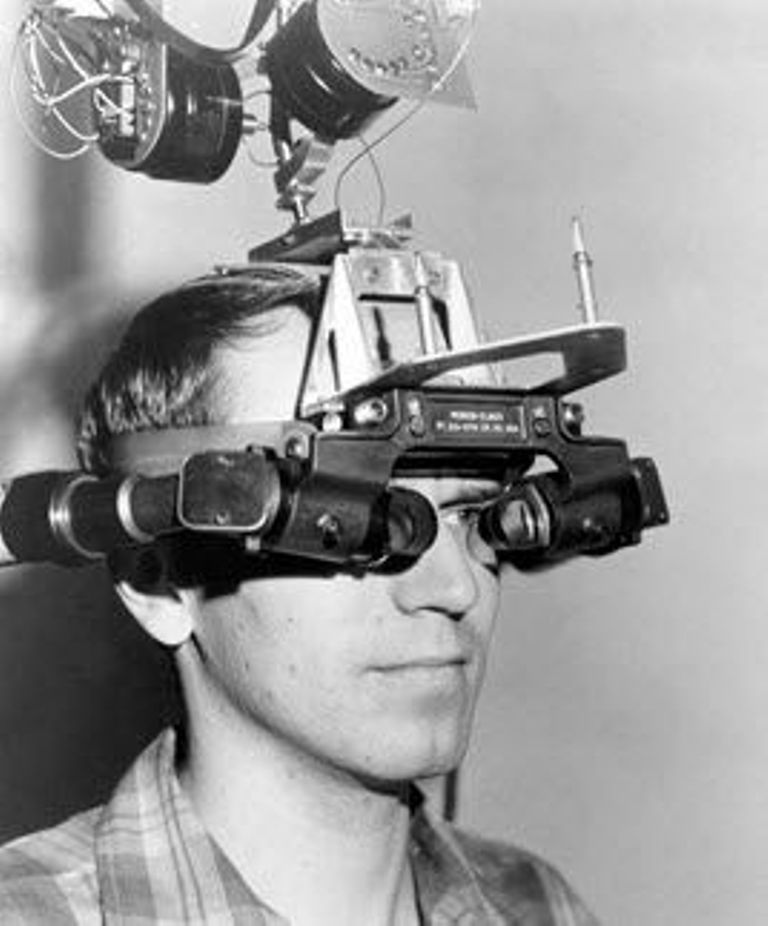
\includegraphics[width=\linewidth]{assets/vr.jpg}
    \end{column}

    \begin{column}{0.45\textwidth}
        Ivan Sutherland creates the first head-mounted 3D display for augmented reality simulations. It is also called "The Sword of Damocles".
    \end{column}
\end{columns}
\end{frame}